\documentclass[12pt]{article}

% PACKAGES
\usepackage[ngerman]{babel}
\usepackage{lmodern} % Schriftart
\usepackage{bookmark} % Für PDF Lesezeichen
\usepackage{caption} % Für \caption*{}
\usepackage{siunitx} % SI-Einheiten
\usepackage{mathtools} % Verbessertes "amsmath" (https://de.overleaf.com/learn/latex/Articles%2FMathtools_-_for_beautiful_math)
\usepackage{xcolor}   % Farbiger Text (https://www.overleaf.com/learn/latex/Using_colours_in_LaTeX)
\usepackage{geometry} % Zur Einstellung des Layouts
\usepackage{titlesec} % Einteilung des Inhalts (https://de.overleaf.com/learn/latex/Sections_and_chapters)
\usepackage{fancyhdr} % Für Kopf-/ und Fußzeilen (https://www.overleaf.com/learn/latex/Headers_and_footers)
\usepackage{parskip} % Änderung von Absätzen und Absatzeinzügen
\usepackage{biblatex} % Verweise und Referenzen
\usepackage{float} % Benötogt für Figuren und Tabellen
\usepackage{graphicx} % Platzhalter Bilder
\usepackage{booktabs} % Tabellen
\usepackage{csquotes} % Recommended package for biblatex
\usepackage{hyphenat}
\usepackage{listings} % for typesetting code
\usepackage{graphicx}
\usepackage{caption}
\usepackage{subcaption}
% SETUP 
\setlength{\headheight}{15.059pt} % Set headheight to at least 14.5pt
\addtolength{\topmargin}{-2.5pt} % Make topmargin smaller to compensate
\sisetup{
  output-decimal-marker={,},
  per-mode=fraction,
  fraction-function=\tfrac,
  separate-uncertainty=true
}

\addbibresource{Ressourcen/V18.bib}
\geometry{ %A4
  a4paper,
  total = {170mm,240mm},
  left = 20mm,
  top = 30mm
}
\pagestyle{fancy}
\captionsetup[figure]{
    justification=centering, % Centered captions
    labelsep=colon, % Separate label and caption with a period
    singlelinecheck=false, % Always center even if the caption is short
    labelfont=bf % Bold captions
}
% COMMANDS
\newcommand{\uproman}[1]{\uppercase\expandafter{\romannumeral#1}} % Römische Zahlen

\sisetup{
  per-mode=fraction,
  fraction-function=\tfrac,
  separate-uncertainty=true,
  output-decimal-marker={,}
}
% DOC
\begin{document}

% HEADER
\begin{titlepage}
  \centering
  \vspace*{1cm}
  
\includegraphics[width=0.5\textwidth]{Ressourcen/tud_logo_schwarz(RGB)}\\
  \vspace*{0.25cm}
  \large\textmd{Fakultät Physik} \\
  \vspace*{6cm}
  \huge \bfseries FP-2024 - Versuch V18\\
  \vspace*{0.25cm}
  \large Germaniumdetektor\\
  \vspace*{0.25cm}
  \large\textmd{\href{mailto:jan.oppoli@tu-dortmund.de}{Jan Oppoli}} \\
  \vfill
  \small\textmd{Versuch durchgeführt am 24. Juni 2024}\\
  \small\textmd{Abgabe erstellt am \today}
\end{titlepage}
\tableofcontents 
\newpage

\section{Zielsetzung}\label{sec:zielsetzung}
Ziel des vorliegenden Versuchs ist es, mithilfe eines hochreinen Germaniumdetektors verschiedene Radioaktive Gammastrahler auf ihre Charakteristika, wie die Vollenergienachweiswahrscheinlichkeit, zu untersuchen.
Nach einer Energiekalibration mittels hinreichend dokumentierter Probe werden die Spektren von sowohl bekannten Materialien, als auch zu bestimmenden Elementen gemessen und ausgewertet.
Aufgrund des hohen Energieauflösevermögens sind Germaniumdetektoren von enormem Wert für die Gamma-Spektroskopie.
\section{Theorie}\label{sec:theorie}
Nachdem zunächst auf die verschiedenen Wechselwirkungen von elektromagnetischer Strahlung mit Materie eingegangen wird, folgt mit diesem Wissen eine Einführung in die Funktionsweise des verwendeten Germaniumdetektors.
\subsection{Wechselwirkungsprozesse von Photonen mit Materie}
Im Wesentlichen spielen drei Effekte eine wesentliche Rolle bei dem Einfall von im Versuch erzeugten Gammaquanten in Materie, wie in \autoref{fig:extinkt} dargestellt ist.
Allgemein kann die Intensität $I$ von Strahlung innerhalb eines Materials abhängig von der Eindringtiefe $x$ mithilfe der Funktion
\begin{align}
  I(x) = I_0\cdot\exp{(-\mu x)}
\end{align}
modelliert werden, wobei $\mu$ Extinktionskoeffizient oder Absorptionskoeffizient genannt wird. Dieser von verschiedenen Materialeigenschaften sowie Strahlungsenergie abhängige Paramater beschreibt, wie stark ein Material die respektive Strahlung abschwächt.
Im Anschließenden wird der zustandekommende Graph erklärt.
\begin{figure}[H]
  \centering
  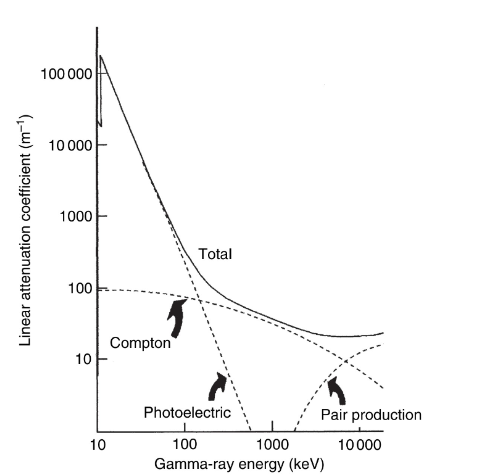
\includegraphics[scale=0.65]{Ressourcen/extinkt.png}
  \caption{Schematischer Verlauf des Extinktionskoeffizienten in Abhängigkeit der Photonenenergie\cite{gilmore}.}
  \label{fig:extinkt}
\end{figure}
\subsubsection{Photoelektrischer Effekt}
Der Photoeffekt beschreibt den Prozess, bei dem ein Gammaquant seine gesamte Energie an ein Hüllelektron eines Atoms abgibt, es herauslöst und das Atom somit ionisiert. Damit es zu diesem Verhalten kommen kann, müssen die Photonen bestimmte Energien, welche mit den Bindungsenergien der Elektronen im Atom übereinstimmen, besitzen.
Der Wirkungsquerschnitt $\sigma$, ein Maß für die Wahrscheinlichkeit eines Wechselwirkungsprozesses, sinkt für den Photoelektrischen Effekt mit steigender Energie, was sich in \autoref{fig:extinkt} in einer linearen Abnahme des Extinktionskoeffizienten $\mu$ widerspiegelt.
Ebenso ist ersichtlich, dass dieser Prozess für Photonenenergien bis zu $\SI{100}{\kilo\electronvolt}$ dominiert.
\subsection{Compton-Effekt}

\section{Aufbau}
\section{Durchführung}\label{sec:durchfuehrung}
\section{Auswertung}\label{sec:auswertung}
\section{Diskussion}\label{sec:diskussion}
\section{Literaturverzeichnis}\label{sec:literaturverzeichnis}
\printbibliography[heading = none]
\newpage

\section{Anhang}\label{sec:anhang}

\end{document}
